\newpage
\section*{Problem 4:}

Figure \ref{fig:problem_4} shows the associated graph $G(A)$ of matrix $A$ along with the steps of the minimum degree algorithm. From these steps, the reordering of the nodes will be $2, 4, 5, 3, 6, 7, 1, 8, 9$



\begin{figure}[!tbh]
\centering        
   \subfloat{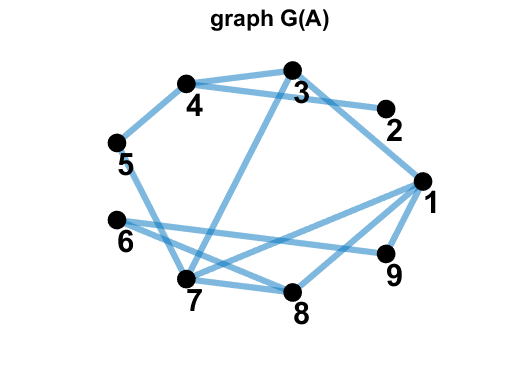
\includegraphics[width=0.33\textwidth]{../code/0.png}}
   \subfloat{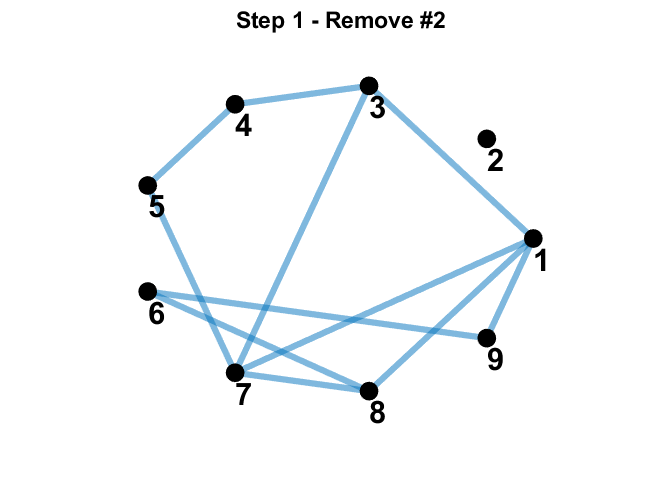
\includegraphics[width=0.33\textwidth]{../code/1.png}}   
   \subfloat{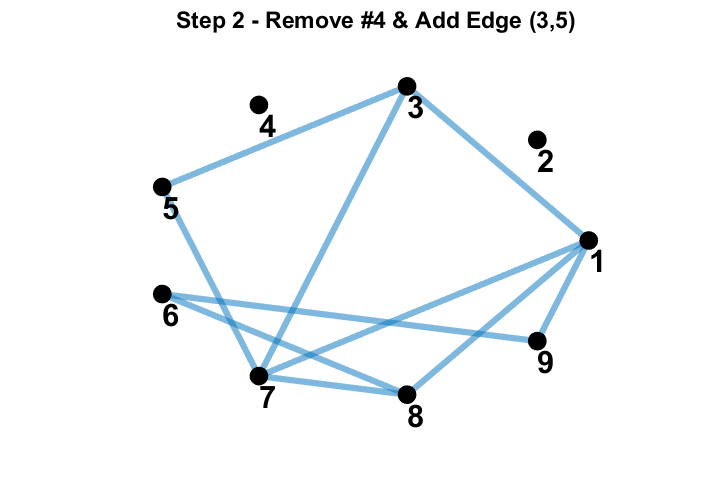
\includegraphics[width=0.33\textwidth]{../code/2.png}}
    
   \subfloat{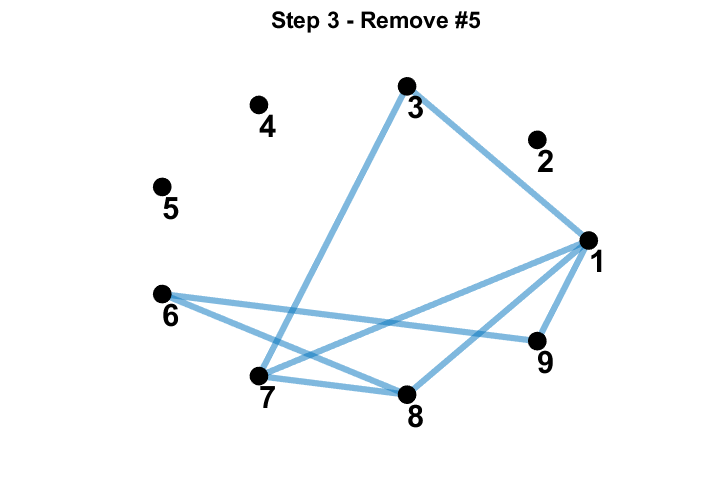
\includegraphics[width=0.33\textwidth]{../code/3.png}}
   \subfloat{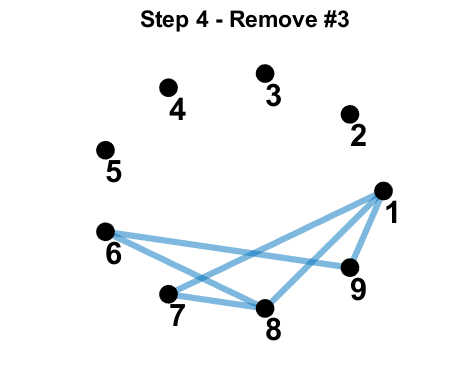
\includegraphics[width=0.33\textwidth]{../code/4.png}}
   \subfloat{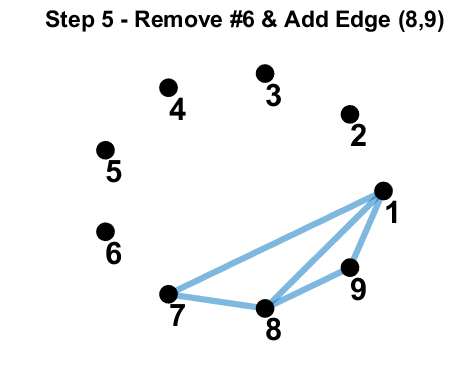
\includegraphics[width=0.33\textwidth]{../code/5.png}}
   
   \subfloat{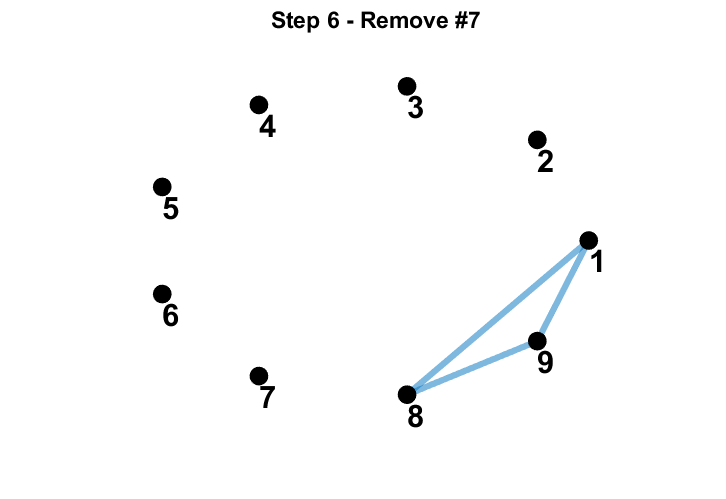
\includegraphics[width=0.33\textwidth]{../code/6.png}}
   \subfloat{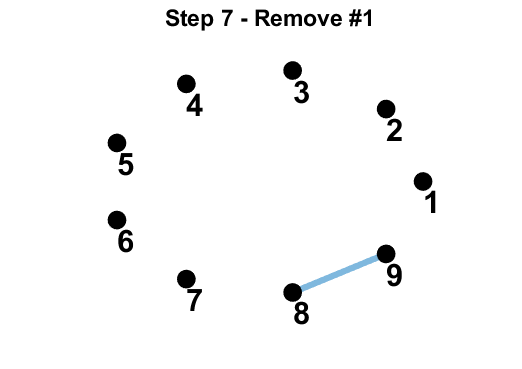
\includegraphics[width=0.33\textwidth]{../code/7.png}}
   \subfloat{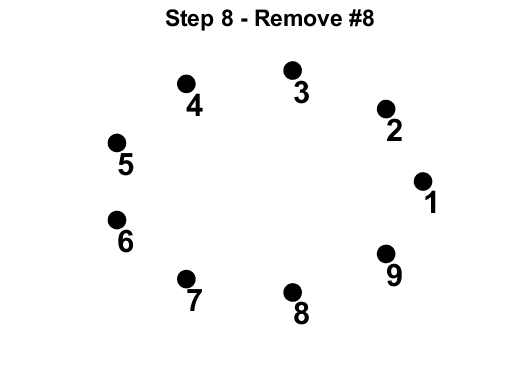
\includegraphics[width=0.33\textwidth]{../code/8.png}}
   \caption{Graph $G(A)$ along with the 8 steps of the minimum degree algorithm applied on it. }
   \label{fig:problem_4}
\end{figure}

\noindent
From the reordering above, the permutation matrix can be constructed such that 

$$
P = 
\begin{bmatrix}
0 & 0 & 0 & 0 & 0 & 0 & 1 & 0 & 0\\
1 & 0 & 0 & 0 & 0 & 0 & 0 & 0 & 0\\
0 & 0 & 0 & 1 & 0 & 0 & 0 & 0 & 0\\
0 & 1 & 0 & 0 & 0 & 0 & 0 & 0 & 0\\
0 & 0 & 1 & 0 & 0 & 0 & 0 & 0 & 0\\
0 & 0 & 0 & 0 & 1 & 0 & 0 & 0 & 0\\
0 & 0 & 0 & 0 & 0 & 1 & 0 & 0 & 0\\
0 & 0 & 0 & 0 & 0 & 0 & 0 & 1 & 0\\
0 & 0 & 0 & 0 & 0 & 0 & 0 & 0 & 1\\
\end{bmatrix}
$$

\noindent
From which, we can compute $P^{T}AP$ to be

$$
P^{T}AP = 
\begin{bmatrix}
* & * & 0 & 0 & 0 & 0 & 0 & 0 & 0 \\
* & * & * & * & 0 & 0 & 0 & 0 & 0 \\
0 & * & * & 0 & 0 & * & 0 & 0 & 0 \\
0 & * & 0 & * & 0 & * & * & 0 & 0 \\
0 & 0 & 0 & 0 & * & 0 & 0 & * & * \\
0 & 0 & * & * & 0 & * & * & * & 0 \\
0 & 0 & 0 & * & 0 & * & * & * & * \\
0 & 0 & 0 & 0 & * & * & * & * & 0 \\
0 & 0 & 0 & 0 & * & 0 & * & 0 & * \\
\end{bmatrix}
$$

\noindent
Applying Cholesky factorization to $P^{T}AP$ we get the following lower triangular matrix where the fill-in elements are shown with $\color{red}{+}$

$$
L = 
\begin{bmatrix}
* & 0 & 0 & 0 & 0 & 0 & 0 & 0 & 0 \\
* & * & 0 & 0 & 0 & 0 & 0 & 0 & 0 \\
0 & * & * & 0 & 0 & 0 & 0 & 0 & 0 \\
0 & * & \color{red}{+} & * & 0 & 0 & 0 & 0 & 0 \\
0 & 0 & 0 & 0 & * & 0 & 0 & 0 & 0 \\
0 & 0 & * & * & 0 & * & 0 & 0 & 0 \\
0 & 0 & 0 & * & 0 & * & * & 0 & 0 \\
0 & 0 & 0 & 0 & * & * & * & * & 0 \\
0 & 0 & 0 & 0 & * & 0 & * & \color{red}{+} & * \\
\end{bmatrix}
$$
